\chapter{Introduction to feedback control}

\todo{
\begin{itemize}
	\item Reference to blog, Hellerstein and Janert
	\item Basics of feedback control
	\item We apply feedback control to computer science
	\item Difference mathematical approach and our approach (also Hellerstein and Janert)
\end{itemize}}

Control is something we deal with every day. Whether it is the temperature in our houses, the number of people in line at the supermarket's checkout or something more critical like the number of neutrons emitted during a nuclear reaction in a reactor, we have to control it to avoid potential chaos.

In software development we too want to have control over the products we both create and use. For example, most applications have a settings menu where the user can alter the application's behavior to their liking; to ensure our code to be working correctly we use compilers, IDEs and automated testing tools that warn us against errors and bugs; Microsoft used to do extensive user studies when introducing new features \cite{meijer2014-embracing-the-hacker-way} and with that control the usability of their product; and last but not least, in cloud computing we want to control the number jobs in a queue and probably scale up or down depending on the amount of jobs in the queue, such that all jobs get executed as fast as possible with spending the least amount of resources.

A common factor in controlling a system is the notion of feedback: you change something in the environment and see how well it adjusts towards your desired outcome. If the lines at checkout get too long, maybe an extra cash register needs to be opened; if your users don't perform well during the user study of your latest features, you should probably revise these features rather than bringing them into production; and when you alter the settings in an application, you check whether the new behavior is more to your desire and maybe fiddle around with them some more.

Controlling a system without the notion of feedback is possible, however this requires a very exact model of the system under control. No external forces that are not part of the model can be allowed to disturb the system. In most cases this model does unfortunately not exist and control has incorporate the system's output to come up with it's next input. If the output is not taken into account, the system can drift off and end up in undesired situations. A nice example of this are Microsoft's user studies: the user's feedback was not taken into account when Office 2007 introduced the "ribbon" to replace the existing user interface and when the start button disappeared in Windows 8 and suddenly every Windows user lost their accumulated muscle memory for commanding the Windows operating system \cite{meijer2014-embracing-the-hacker-way}.

In physics and engineering, feedback control is a commonly used technique and also is fully backed by mathematics. A series of equations and theorems such as Laplace Transforms and differential equations describe the abstract behavior of a feedback controlled system and allows to evaluate its outcome after running it for a certain time and with a certain input \cite{hellerstein2004-feedback, janert2013-feedback}. These theorems and equations are so usable in science because everything else is described in the `language of mathematics' as well. We have known the differential equations to Newton's law of cooling, damped harmonic oscillators and so forth for centuries, as well as their Laplace Transforms, which are needed for the `feedback equations'.

This is all in contrast to the current situation in computer science. Although proven to be very effective in physics, computer science has not yet widely adopted the techniques of feedback control. Instead, complex algorithms are written to control a web cache or do cloud scaling. Although some work has been done \todo{citation needed}, it is surprising to find that such a simple and effective technique (we will get into this more later) is mostly ignored.

A potential reason for this lack of using feedback control lies in the fact that computer science does not yet fully understand the whole mathematical background of the datastructures and applications that they are using and creating. Given this lack of understanding, we are not yet able to describe to which laws our datastructures and application obey. What would be the equivalent of Newton's laws for a web cache \cite{janert2013-feedback}? Only recently some work has been done on understanding the mathematics behind this \cite{beckmann2015-cache-calculus} and we may very well see more of this in the future, which will eventually enable computer science to create a more formal model.

The lack of applying feedback control in computer science is also reflected in this technique commonly not being taught in university degree computer science education. Although it is one of standard courses in physics and engineering studies, it is not at all present in the computer science curricula. And in the rare occasions it is taught, it is done in a way that a physics student would learn about it, namely as yet another maths course, even though this way of treating feedback control in computer science is not really applicable!

\section{Overview}
In general a system is controlled by feedback when its next input value is (partially) determined by its previous output(s). The reason for taking the previous output into account while coming up with a next input is due to external forces that may impacting the system in unexpected ways. These external forces do not come regularly, are not predictable and are also not equally strong each time, hence a notion of uncertainty in the system's behavior occurs. Due to this uncertainty, a model that accurately calculates the system's next input either does not exist or would be too complex. The solution for incorporating the uncertainty from external forces is to use a feedback cycle around the system: the system's output (affected by both the system's input and any external forces) is measured and compared to a desired reference value, after which their difference is transformed into the system's next input.

Important to mention here early on is that controlling a system with a feedback cycle is not a solution to optimization problems. Tasks like ``\textit{Make the flow through the system as large as possible}'' cannot be accomplished with feedback loops \cite{janert2013-feedback}, as they compare the system's current output with a known reference value. Tasks like this require some kind of optimization strategy that determines the reference value, after which a feedback loop can be used to bring and keep the system's output in this desired state.

The input and output of a feedback controlled system are not to be confused with the actual input and output of this system. The air conditioning or heating system has an actual output of hot or cool air, whereas the feedback system's output can be any other measurable metric such as the new temperature after the actual output is applied or the temperature difference caused by the actual output. The input and output of a feedback controlled system are often referred to \textit{control input} and \textit{control output}.

\subsection{Calculating the next control input}
Every time the control output produces a new value, it is compared to a reference value or \textit{setpoint} for it to calculate the \textit{tracking error} as the deviation of the control output from the setpoint:

\begin{equation} \label{eq:tracking-error}
\text{tracking error} = \text{setpoint} - \text{control output}
\end{equation}

This tracking error is then transformed into the next control input by the \textit{controller}. When the tracking error is positive (thus the control output is less than the setpoint), the controller has to produce a new control input that ultimately raises the control output to the same level as the setpoint, such that the tracking error becomes zero. Of course this depends on the \textit{directionality} of the system: for some systems the control input needs to be lowered for the system output to be raised. The controller must be able to make this distinction and therefore has to know the directionality of the system. For example, a heating system requires the controller to \emph{raise} the control input to get a higher temperature, whereas a cooling system requires the controller to \emph{lower} the control input to get a higher temperature.

Besides the directionality, the controller also needs to decide on the magnitude of the correction. If the magnitude is too high, the controller could overcompensate and turn a positive tracking error into a negative tracking error and vice versa, causing the system to oscillate between two states. The worst situation occurs when the negative tracking error caused by the overcompensation of the positive tracking error is larger than the positive tracking error: this results in an ever growing amplitude of the oscillation, which eventually makes the whole system unstable and in the end causes it to blow up.

On the other hand, the magnitude can be too low, causing the controller to undercompensate. This causes tracking errors to persist for a longer time than necessary and makes the system respond slow to disturbances. Although this is less dangerous than instability, this slow behavior is unsatisfactory as well.

In general we require the controller to take in a tracking error and come up with a new control input such that the tracking error will go to zero as soon as possible. For this it turns out that the controller does not need to know anything about the controlled system, but only requires information about the directionality of the system and the magnitude of the correction.

\subsection{Architectural overview}
The architecture of a feedback system is usually depicted as a set of boxes connected with arrows. This way we get a quick overview of the design without worrying about the exact implementation of the various components. The general architecture of a feedback system as discussed above is shown in \autoref{fig:feedbackArchitecture}. Notice that here the control output is negated on the way back and is then added to the setpoint in order to calculate the tracking error. This is common practice as some more preprocessing is required before comparing the control output with the setpoint. For example, the output may contain noise which needs to be smoothened by some kind of filter. Of course preprocessing steps will also be drawn in this overview if applicable.

\begin{figure}[H]
	\begin{center}
		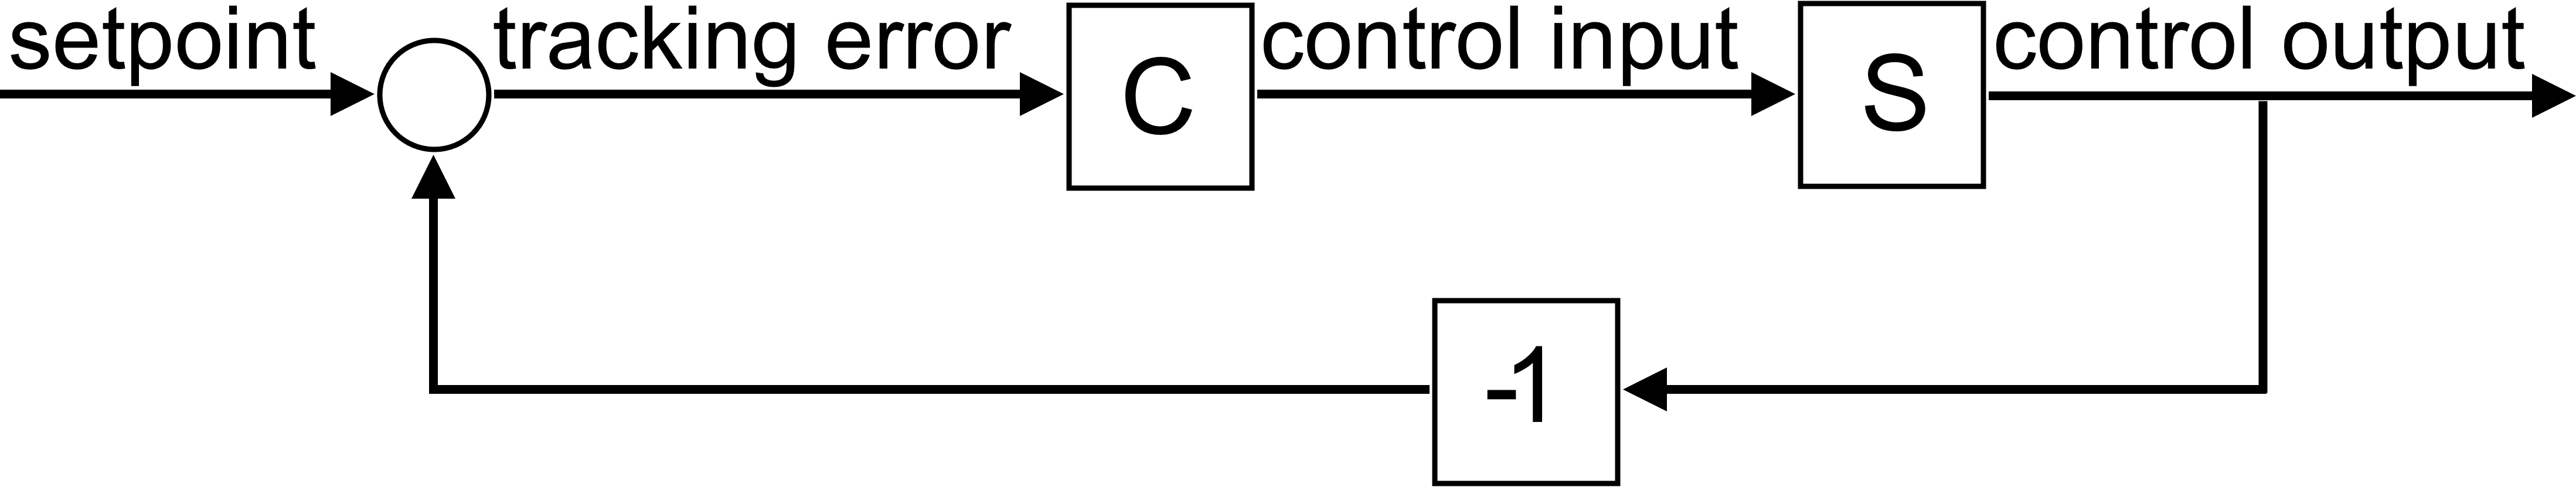
\includegraphics[width=0.85\textwidth]{figures/FeedbackBig.png}
	\end{center}
	\caption{The architecture of a feedback control system}
	\label{fig:feedbackArchitecture}
\end{figure}

Besides these filters, a controller may consist of multiple components by itself. When using an incremental controller, only the difference in the control input is outputted. For the actual input we need to maintain a running sum of all the previous controller outputs and in that way calculate the actual control inputs. Usually these extra steps are also depicted in the architectural overview as extra boxes and arrows.


\section{Different types of controllers}
The control input in a feedback system is the value that tells the system under control to behave slightly different than it did and possibly incorporating external disturbances on the system in a better way. As discussed in the previous section, this control input value is computed in the controller part of the feedback system. Although one might expect differently, the controller itself does not turn out to be very smart or know a whole lot about the system under control. As mentioned before, a controller in fact only needs to know about directionality of the system and the magnitude of the correction for it to work just fine. There are a number of controllers that only need these two pieces of information and that are commonly used in physics, mechanics and electronics.

\subsection{On/Off control}
The most simple controller one can think of is just an on/off switch. Whenever the tracking error is positive, the controlled system is turned on and when the tracking error becomes negative it is turned off again\footnote{Of course this is dependent upon the directionality of the system under control.}. For simple systems this kind of control will suffice, although it will not be a very effective approach.

An application of this kind of control might be a air conditioning system that turns on when the temperature exceeds a preset level. In this example the control output is the current temperature in the room, the setpoint is the preset temperature, the control input is a boolean value which determines whether the system should be on of off and the directionality of the system is negated. Imagine the temperature initially being much too high, causing the air conditioning to turn on right away. After a certain amount of time the temperature reaches the desired setpoint (the tracking error becomes zero), hence the system will shut down. Shortly after the air conditioning system is shut down, the temperature starts increasing again. This immediately causes a deviation from the setpoint, forcing the air conditioning to turn on again. Soon enough the temperature is low enough again for the system to be turned off, after which the cycle starts all over again. Of course this kind of behavior is very annoying to everyone working in this room, as the air conditioning continuously turns off and on again. Besides that, this behavior costs an unnecessary amount of energy for turning the system on and off, which is not really desirable either.

Obviously this behavior is caused by the controller that dictates to turn off the system whenever the setpoint is met. Due to external disturbances such as whether conditions the feedback system is off track soon again, which causes the controller to decide to turn the controlled system back on.

Small improvements that are often used in these kinds of systems are introducing a dead zone or Schmitt trigger, which causes the system to continue with the same corrective action until a certain threshold or a certain amount of time is exceeded. This prevents the controller from overreacting on sudden and short spikes in the control output. In the case of the air conditioning an addition such as this will cause the controller to not immediately send a `turn off signal' when the setpoint is zero and will not activate the system with the slightest deviation, but instead waits a little longer until a threshold is exceeded before activating or deactivating the system again.

\subsection{Proportional control}
Another simple controller 


